% 109-18(인쇄 109쪽) — 힌트의 정규분포곡선: m-σ 부터 m 까지의 넓이(P(m-σ≤X≤m))를 색칠한 그림.
% 스캔 화질이 낮아 TikZ 로 다시 그림. 라벨은 원문에 있는 것만(m-σ, m, x) · 구하는 확률은 그림에 적지 않는다.
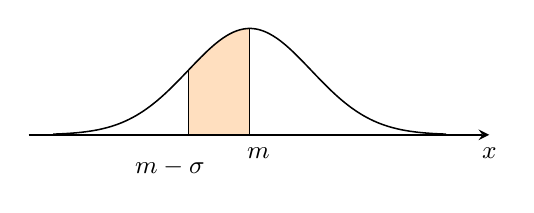
\begin{tikzpicture}[x=0.78cm, y=1.35cm, line width=0.55pt, font=\small]
  \fill[orange!25] plot[domain=-1:0, samples=40, smooth] ({\x},{exp(-\x*\x/2)}) -- (0,0) -- (-1,0) -- cycle;
  \draw[->, >=stealth, line width=0.7pt] (-3.6,0) -- (3.9,0) node[below=1pt] {$x$};
  \draw plot[domain=-3.2:3.2, samples=110, smooth] ({\x},{exp(-\x*\x/2)});
  \draw[line width=0.4pt] (-1,0) -- (-1,{exp(-0.5)});
  \draw[line width=0.4pt] (0,0) -- (0,1);
  \node[below=1pt] at (0.14,0) {$m$};
  \node[below=5pt] at (-1.3,0) {$m-\sigma$};
\end{tikzpicture}
